\documentclass{article}

\usepackage{amsmath, amsthm, amssymb}
\usepackage[round]{natbib}
\usepackage{algorithm}
\usepackage{algpseudocode}
\usepackage[left=2.5cm, right=2.5cm, top=3cm, bottom=3.00cm]{geometry}
\usepackage{array}
\usepackage{booktabs}
\setlength{\heavyrulewidth}{1.5pt}
\setlength{\abovetopsep}{4pt}

% The line below tells R to use knitr on this.
%\VignetteEngine{knitr::knitr}

\title{Elliptical Slice Sampling}
\author{Francesca Panero \and Xuewen Yu}

\usepackage{Sweave}
\begin{document}
\Sconcordance{concordance:my_vignette.tex:my_vignette.Rnw:%
1 14 1 1 0 275 1}


\maketitle

\begin{abstract}
In this project, we presented the R package `ESS', which provides an implementation of the Elliptical Slice Sampling method presented by Murray, Adams and MacKay in 2010 $\cite{MAM}$. We validated this algorithm on the simplest senario of Gaussian regression model and compared it with Metropolis Hastings algorithms on two Gaussian Process based likelihood models.
\end{abstract}

\section{Introduction}

Slice sampling was introduced by Neal in 2003 \cite{Neal2003} in the homonym paper published in the Annals of Statistics. Neal's idea was to present a new approach to sample from a probability density function, that tried to overcome some drawbacks of the two major MCMC methods of sampling: the Gibbs sampler and the Metropolis Hastings method.

The aim of these three methods is to sample from a probability density function from which we are not able to sample directly. Their basic idea is to construct a Markov chain that have as stationary distribution the target one we care about, and samples from this chain will eventually come from the desired distribution. 

%Gibbs sampler exploits the possibility of sampling from the full conditional density functions of each parameter given all the others (that are usually simpler to deal with than the original joint distribution), since the complete vector of parameters will eventually be sampled from the joint distribution of these. No tuning of parameters of the chain is required, but we must be able to sample from these conditional distributions in order to implement the method, and sometimes this could not be the case. Nevertheless, some algorithms to overcome this problem have been proposed, in particular ARS (adaptive rejection sampling) and MARS (adaptive rejection Metropolis sampling).
%Metropolis Hasting, instead, initializes the chain with a value sampled from a proposal distribution from which we are able to sample from and that attains some nice links with the target distribution. This sample can be accepted or rejected according to a probability that depends on the likelihood of the new candidate point and the previous one. This method presents some scale parameters for which there does not exist a certain rule of decision; moreover, the proposal distribution does not always come from a straightforward reasoning.

%Slice sampling tries to overcome these flaws in the previous methods. 
The basic idea of slice sampling lies in the fact that if we want to sample $x$ from a distribution $p(x)$ that is proportional to a certain function $f(x)$, it would be sufficient just to sample uniformly from the area below $f(x)$.
By defining an auxiliary random variable $y$, we exploit Gibbs sampler to sample from the two full conditional distributions. In particular, $y|x$ is distributed as an $Uniform(0,f(x))$ and $x|y$ is distributed as an uniform on the so called slice $S=\lbrace x: y<f(x)\rbrace$. The joint density of $x$ and $y$ is, then $$p(x,y)=\begin{cases}1/Z\quad&\text{ for }0<y<f(x)\\0\quad&\text{ otherwise}\end{cases}$$where $Z=\int f(x)dx$. From this it can easily be seen that $p(x)=\int_0^{f(x)} p(x,y)dy=(1/Z)f(x)$ as desired. 
%Sampling on the slice can be difficult, and it is sometimes substituted with some update for $x$ which leaves invariant the uniform distribution.

Based on this idea, Murray, Adams and Mackay proposed Elliptical Slice Sampling for multivariate Gaussian priors and indicated the advantage of this new method over MCMC methods in terms of computational complexity and performance of the sampled Markov chains \cite{MAM}. This project aims to implement Elliptical Slice Sampling in R and assess the performance of Elliptical Slice Sampling on Gaussian regression model and Log Gaussian Cox process model.

\section{Elliptical Slice Sampling}

Elliptical Slice Sampling is a particular case of MCMC methods that avoids the tuning of parameters, simpler and often faster than other methods to sample from the posterior distribution of models with multivariate Gaussian prior.

Let $\mathbf{f}$ be the vector of latent variables distributed as a Gaussian distribution with zero vector mean and covariance matrix $\Sigma$: $$\mathbf{f}\sim\mathcal{N}(\mathbf{f};\mathbf{0}, \Sigma)=|2\pi\Sigma|^{-1/2}\text{exp}\left(-\frac{1}{2}\mathbf{f}^T\Sigma^{-1}\mathbf{f}\right)$$ Let $$L(\mathbf{f})=p(\text{data}|\mathbf{f})$$ be the likelihood function. Our target distribution is the posterior of this model: $$p^*(\mathbf{f})\propto \mathcal{N}(\mathbf{f};\mathbf{0}, \Sigma)L(\mathbf{f}).$$

Neal, in 1999 \cite{Neal}, introduced the idea of a Metropolis-Hastings algorithm for this type of problems, by proposing as new state 
$$\mathbf{f^{'}}=\sqrt{1-\epsilon^2}\mathbf{f}+\epsilon\pmb{\nu},\qquad\pmb{\nu}\sim\mathcal{N}(\mathbf{0}, \Sigma)$$ where $\epsilon\in[-1,1]$ is a step-size parameter, and its varying defines half of an ellipse, having $\pmb{\nu}$ fixed. When $\epsilon=0$ we are resampling the same value. The probability of accepting the move is $$p(\text{accept})=\text{min}(1,L(\mathbf{f^{'}})/L(\mathbf{f}))$$ otherwise the next state is still $\mathbf{f}$. A drawback of this algorithm is that $\epsilon$ needs to be tuned so that the Markov chain can mix efficiently. A representation of the whole ellipse gives a richer choice of updates, so we will exploit: $$\mathbf{f^{'}}=\pmb{\nu}\text{sin}\theta+\mathbf{f}\text{cos}\theta$$ that represents the ellipse centered in the origin of the axes and passing through $\mathbf{f}$ and $\pmb{\nu}$, and $\theta$ is a new step-size parameter.

To avoid the tuning of the parameter, the idea is to augment the prior to make $\theta$ a random variable and sample it exploiting the slice sampling. The augmented model becomes
\begin{align*}
\pmb{\nu}_0&\sim\mathcal{N}(\mathbf{0},\Sigma)\\
\pmb{\nu}_1&\sim\mathcal{N}(\mathbf{0},\Sigma)\\
\theta&\sim \text{Uniform}[0,2\pi]\\
\mathbf{f^{'}}&=\pmb{\nu}_0\text{sin}\theta+\pmb{\nu}_1\text{cos}\theta
\end{align*}
which assures that the distribution of $\bf{f}$ is always $\mathcal{N}(\mathbf{0},\Sigma)$. The new target distribution is $$p^*(\pmb{\nu}_0,\pmb{\nu}_1,\mathbf{f})\propto\mathcal{N}(\pmb{\nu}_0;\mathbf{0},\Sigma)\mathcal{N}(\pmb{\nu}_1;\mathbf{0},\Sigma)L(\mathbf{f}(\pmb{\nu}_0,\pmb{\nu}_1,\theta))$$
The slice sampling exploits the following algorithm:\\

\begin{algorithm}
\caption{ESS Algorithm}\label{ess}
\hspace*{\algorithmicindent} \textbf{Input}: $\mathbf{f},\,\text{log}L$ \\
\hspace*{\algorithmicindent} \textbf{Output}: $\mathbf{f^'}\sim p^*(\mathbf{f})$ 
\begin{algorithmic}[1]
%\Procedure{Euclid}{$a,b$}
  \State Sample from $p(\pmb{\nu}_0,\pmb{\nu}_1,\theta|\pmb{\nu}_0\text{sin}\theta+\pmb{\nu}_1\text{cos}\theta=\mathbf{f})$:
\begin{align*}
\theta &\sim\text{Uniform}[0,2\pi]\\
\pmb{\nu}&\sim\mathcal{N}(\mathbf{0},\Sigma)\\ 
\pmb{\nu}_0 &\leftarrow\mathbf{f}\text{sin}\theta+\pmb{\nu}\text{cos}\theta\\
\pmb{\nu}_1 &\leftarrow\mathbf{f}\text{cos}\theta-\pmb{\nu}\text{sin}\theta
\end{align*}
  \State Sample $\theta$ using slice sampling on $p^*(\theta|\pmb{\nu}_0,\pmb{\nu}_1)\propto L(\pmb{\nu}_0\text{sin}\theta+\pmb{\nu}_1\text{cos}\theta)$ 
  \State $\mathbf{f^{'}}=\pmb{\nu}_0\text{sin}\theta+\pmb{\nu}_1\text{cos}\theta$
%\EndProcedure
\end{algorithmic}
\end{algorithm}

To avoid proposing $\pmb{\nu}_{0}$ and $\pmb{\nu}_{1}$ in every iteration of the algorithm and to shrink the range of $\theta$ after every iteration, Murray, Adams and MacKay \cite{MAM} 
suggested a mature algorithm as follows:

\begin{algorithm}
\caption{Neater ESS Algorithm}\label{ess*}
\hspace*{\algorithmicindent} \textbf{Input}: $\mathbf{f},\,\text{log}L$ \\
\hspace*{\algorithmicindent} \textbf{Output}: $\mathbf{f^'}\sim p^*(\mathbf{f})$ 
\begin{algorithmic}[1]
\State Sample $\pmb{\nu}\sim\mathcal{N}(\pmb{\nu};\mathbf{0},\Sigma)$ (this defines the ellipse centered in the origine passing through $\mathbf{f}$ and $\pmb{\nu}$).
\State Define the slice by sampling the height $y$:
\begin{align*}
u &\sim\text{Uniform}[0,1]\\
\text{log}y &\leftarrow \text{log}L(\mathbf{f})+\text{log}u
\end{align*}
\State Define the bracket for the angles:
\begin{align*}
\theta &\sim\text{Uniform}[0,2\pi]\\
[\theta_{\text{min}},\theta_{\text{max}}]&\leftarrow [\theta-2\pi,\theta]
\end{align*}
\State Propose a new status $\mathbf{f^{'}}\leftarrow\mathbf{f}\text{cos}\theta+\pmb{\nu}\text{sin}\theta$
\If{$\text{log}L(\mathbf{f^{'}})>\text{log}y$}
    \State Accept: \textbf{return} $\mathbf{f^{'}}$
\Else{ Shrink the bracket:}
    \If{$\theta<0$} $\,\theta_{min}\leftarrow\theta$ 
    \Else $\,\theta_{max}\leftarrow\theta$
  \State $\theta\sim\text{Uniform}[\theta_{min}, \theta_{max}]$
  \State Go to 4.
\end{algorithmic}
\end{algorithm}

\begin{figure}
    \centering
    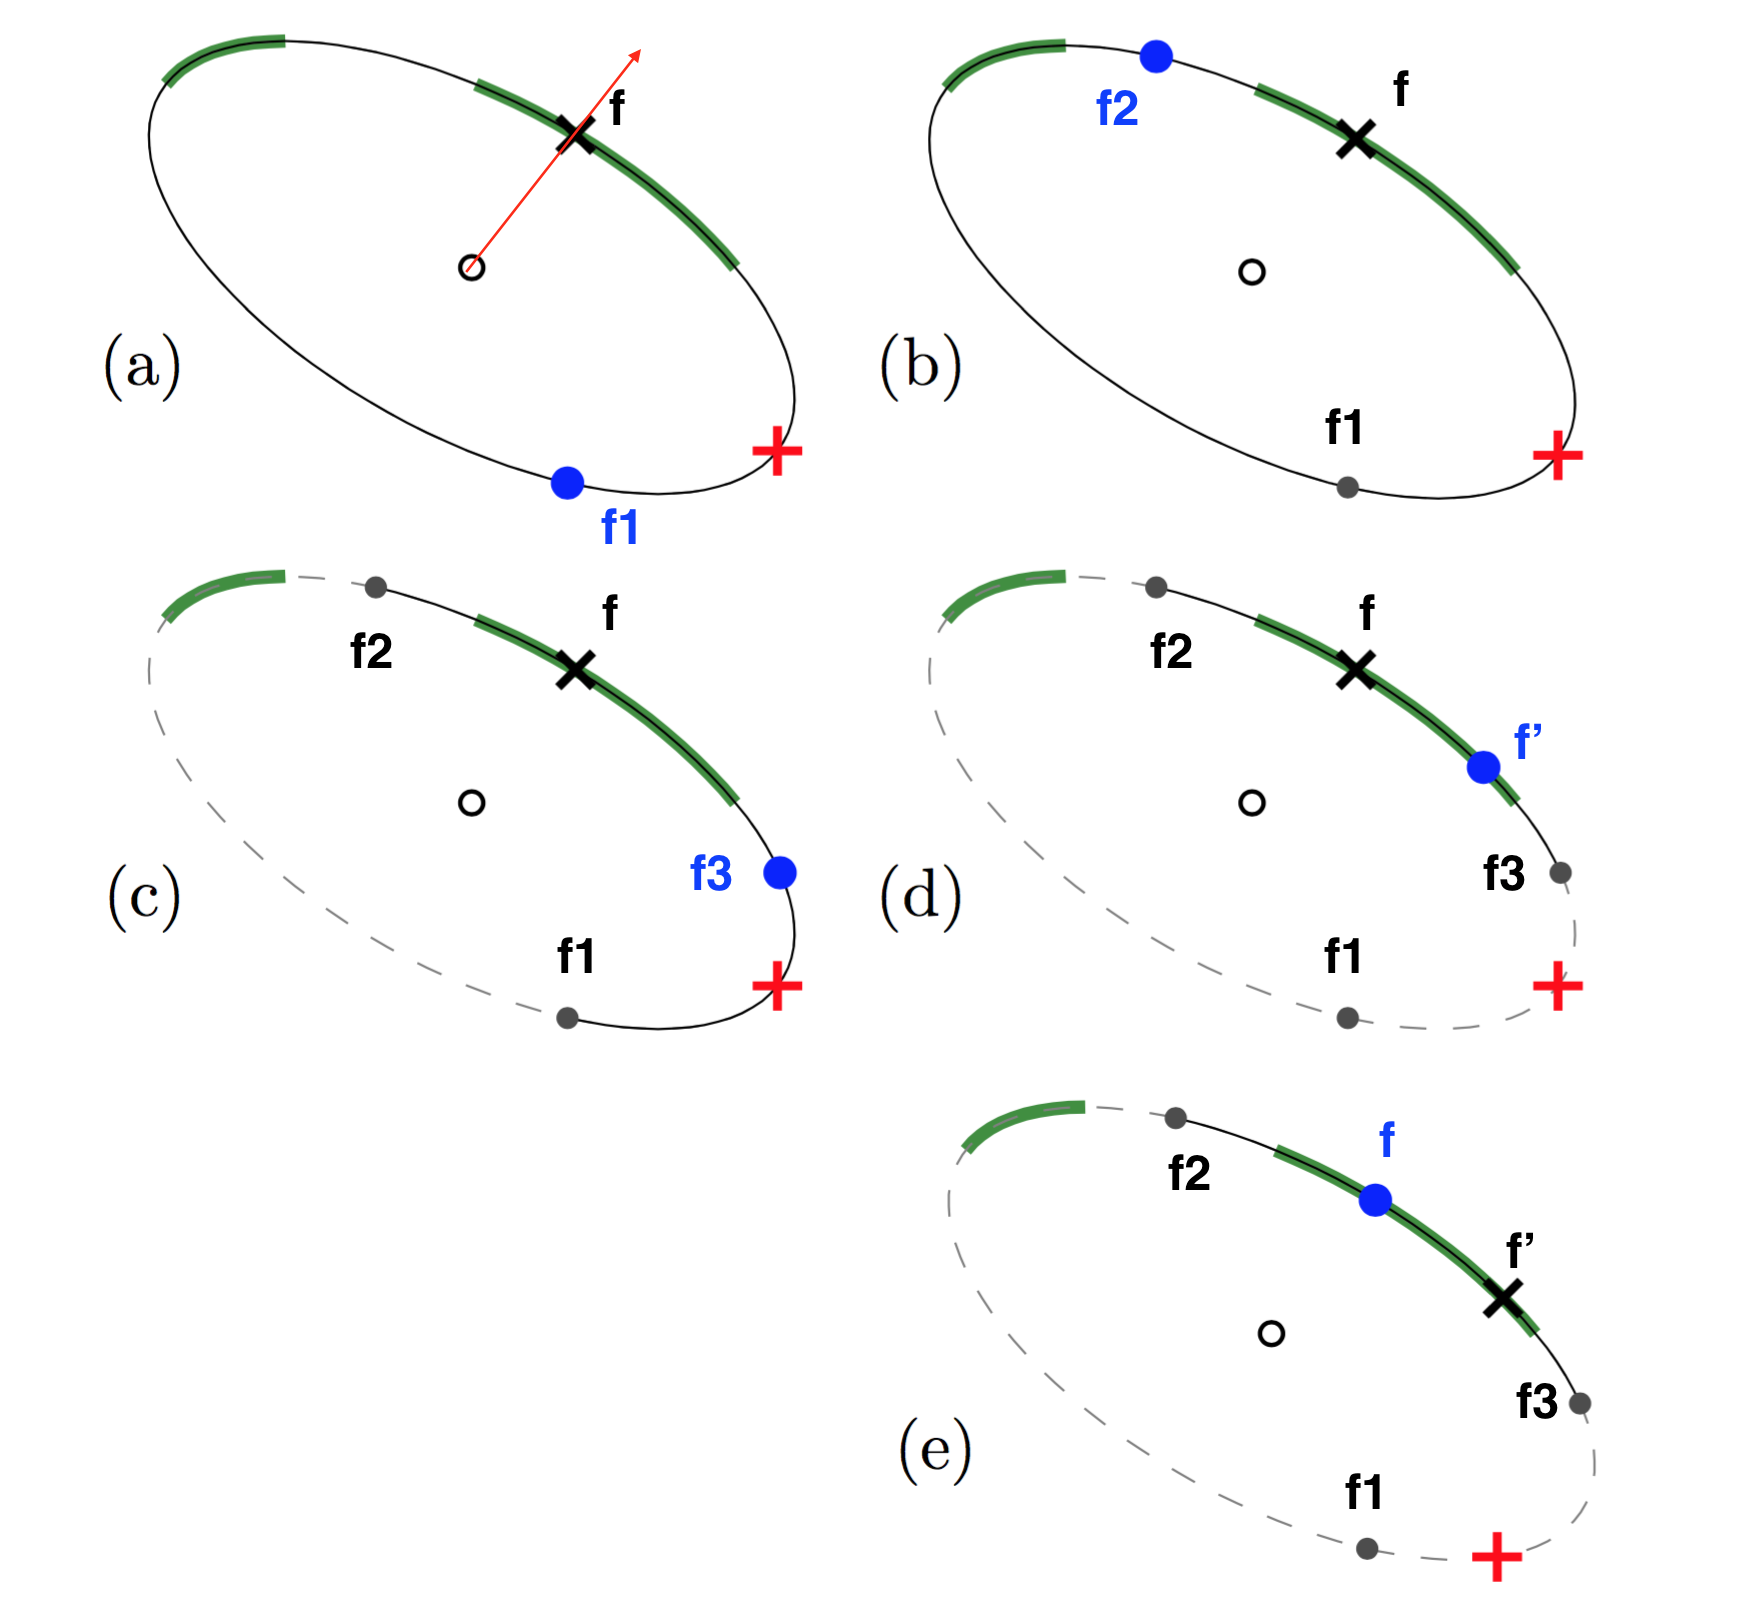
\includegraphics[width = 10cm,height = 8cm]{essfig.png}
    \caption{(a)-(d): Implementing the algorithm by inputting $\bf{f}$, which is denoted by black cross, and update to $\bf{f'}$. The red cross represents the auxiliary variable $\bf{\nu}$, green slice represents the likelihood threshold, blue points are the new proposal in each step, and solid lines are the range that $\theta$s are sampled from. (e) is the reverse procedure proposing $\bf{f}$ back from $\bd{f'}$, where $\bf{\nu'}$ is the red cross.}
\end{figure}

An example of updating $\bf{f}$ to $\bf{f'}$ by implementing this algorithm is shown in Figure 1. $\bf{f}$ is the location where $\theta = 0$. The four proposals are $\bf{f_1}, \bf{f_2}, \bf{f_3}$ and $\bf{f_4}$, where $\bf{f_4} = \bf{f'}$. These states correspond to angles $\theta_k$ $k=1,...,4$. The range that $\theta$s are sampled from shrinks during the implementation of the algorithm such that $\bf{f}$ is always included. The update stops when the proposed new state lies on the green slice, i.e. the range of likelihood satisfying step 5 in the algorithm. This process is reversible and original state $\bf{f}$ can be reached, as shown in (e). When we update the state from $\bf{f'}$, $\theta = 0$ at this point. A rotation of $-\theta_4$ will return back to the original state.


\section{Experiments}
In this section, we will validate the elliptical slice sampling algorithm on 2 models: Gaussian regression and Log Gaussian Cox process, and compare this algorithm with the Metropolis-Hastings algorithm adapted by Neal \cite{Neal}.
  
\subsection{Model Description}
\subsubsection{Gaussian Regression}

Observations $y_n$ are drawn from Normal distribution with mean $f_n$ and variance $\sigma_n^2$, for $n = 1,...,N$. Let $N$ denote the sample size, $D$ denote the number of dimensions. $\bf{f}$ $= (f_1,...,f_N) \sim{N(0,\Sigma)}$. To simulate $\bf{f}$, we define the covariance matrix as 
\begin{equation}
\Sigma_{i,j} = \sigma_{f}^{2}\text{exp}\left(-\frac{1}{2}\sum_{d=1}^{D}(x_{d,i} - x_{d,j})^2/l^2\right)
\end{equation}
The covariance matrix $\Sigma$ is computed by inputing $\mathbf{X}=[\mathbf{x}_1,...,\mathbf{x}_N]^{'}$, which is a $D\times{N}$ matrix where the column vector $\bf{x}_n$, $n = 1,...,N$, are the input $D$-dimensional vectors that will be drawn from a $D$-dimensional unit hypercube for all $n$. 
Fixing $l$ (called ``lengthscale" parameter), $\sigma_{f}^2$ and $\sigma_{n}^2$, we can generate $f_n$ and therefore simulate observations $y_n$, since $\mathbf{y}|\mathbf{f}\sim\mathcal{N}\left(\mathbf{f},\sigma_n^2\mathbf{I}\right)$and therefore their likelihood function as a function of $\bf{f}$ looks like:
\begin{equation}
L_r(\mathbf{f}) = \prod_{n=1}^{N} \mathcal{N}(y_n;f_n,\sigma_n^2)
\end{equation}


\subsubsection{Log Gaussian Cox process}
  Cox process is a "doubly stochastic" Poisson process with a stochastic intensity measure \cite{Moller}. 
  Log Gaussian Cox process is introduced by Moller \cite{Moller} 
  as the Cox process where the logarithm of the internsity function is a Gaussian process. Mathematically, let $y_n$ denote the observations. Then $y_n \sim{Poisson(\lambda_n)}$ with mean $\lambda_n$. The intensity function can be estimated given the log Gaussian Cox process observation within a bounded subset. This means we can partition the space finitely into $N$ bins and $y_n$ is the number of events in bin $n$ for all $n = 1,...,N$. We assume that every bin has a constant intensity function $\lambda_n$. Let $m$ be the offset to the log mean $\lambda_n$, and define it as the sum of the mean log-intensity of the Poisson process and the log of the bin size \cite{MAM}. 
  \begin{equation}
  y_n|f_n \sim{Poisson(exp(f_n + m))}
  \end{equation}
  \begin{equation}
  \bf{f} \sim{N(0,\Sigma)}
  \end{equation}
  
  $\Sigma$ is defined in Equation (7). Then the likelihood of $\bf{y}$ is:
  \begin{equation}
  L_p(\bf{f}) = \prod_{n=1}^{N}\frac{\lambda_{n}^{y_{n}} exp(-\lambda_n)}{y_n!}, \lambda_n = e^{f_n+m}
  \end{equation}
  
\subsection{Implementation and Results}
\subsubsection{Gaussian Regression}

Let $l=1$, $\sigma_{f}^2 = 1$, $\sigma_{n}^2 = 0.3^2$. Firstly, we validate the Elliptical Slice Sampling algorithm on Gaussian regression model when $\bf{f}$ is bivariate Normal variable. In this case, let $N = 2$ and $D = 1$ such that $\{\bf{x}_n\}_{n=1}^{2}$ is one dimensional. Since both prior distribution and likelihood function are Gaussian, the posterior distribution of $\bf{f}$ should be Gaussian. We perform Henze-Zirkler's test to assess whether the outputs follow Bivariate Normal distribution. This is based on the measure of distance, which is nonnegative, between the characteristic function of the multivariate normality and the empirical characteristic function. The distribution of the test statistic is approximately log normal. We achieved a p-value much larger than 0.05, which indicates that there is no strong evidence to reject the null hypothesis that the outputs of the algorithm follows multivariate normal distribtuion. We can visualise the distribution of outputs in Figure 1. As a necessary condition for mutivariate normality, each variable should have normal distribution. We confirm this condition from QQ-plot. 

%\begin{figure} [h!]
%\centering
%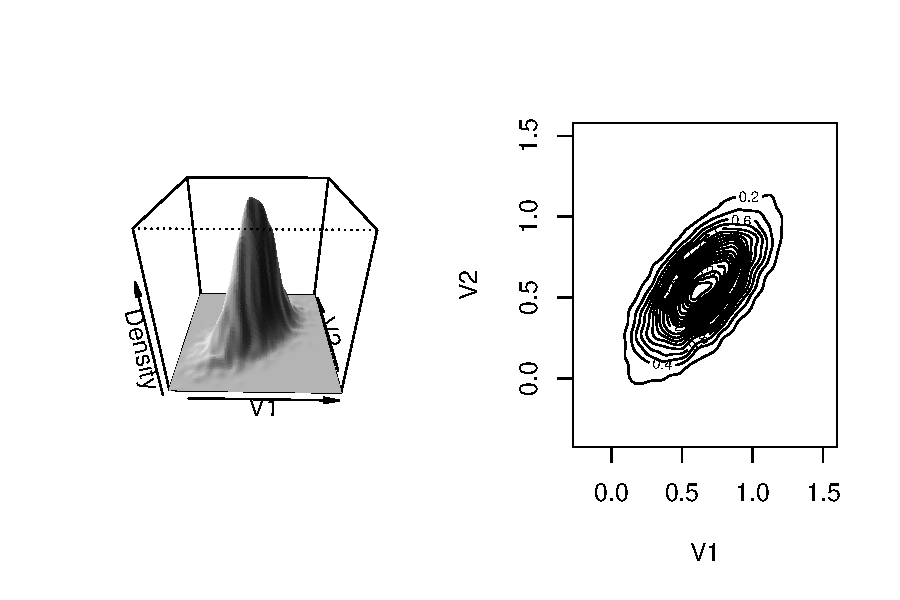
\includegraphics[width = 10cm]{3dplot.pdf}
%\caption{Perspective (left) and Contour (right) plots for bivariate outputs}
%\end{figure}
%\begin{figure} [h!]
%\centering
%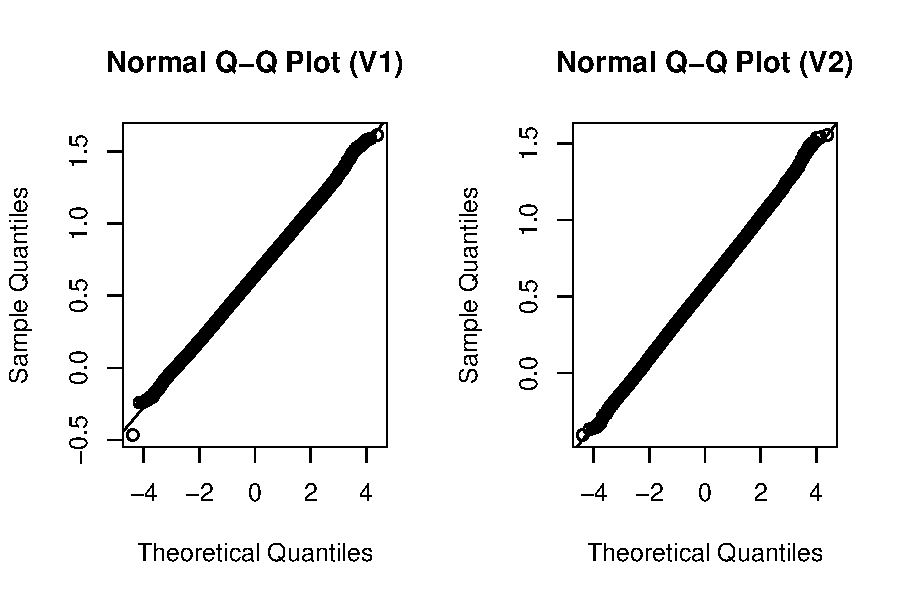
\includegraphics[width = 10cm]{qqplot.pdf}
%\caption{QQ plot of $f_1$ and $f_2$ from Elliptical Slice Sampling algorithm }
%\end{figure}

Then we assess the performance of the algorithm on Gaussian regression when $N=200$, i.e. $\bf{f}$ is 200-dimensional. As stated in the model description section, $\bf{f}$ can be generated by inputing $X$ to covariance matrix. So we first simulated datasets $X$. In order to compare the performance of algorithm for different dimensions, i.e. $D$, of feature vectors, 2 synthetic datasets $X_1$,$X_10$ will be simulated with $D = 1,10$ respectively. This will give different distribution of prior distribution of $\bf{f}$. Denote the observations simulated from these two cases as $R1$ and $R10$ respectively.
%\begin{figure} [h!]
%\centering
%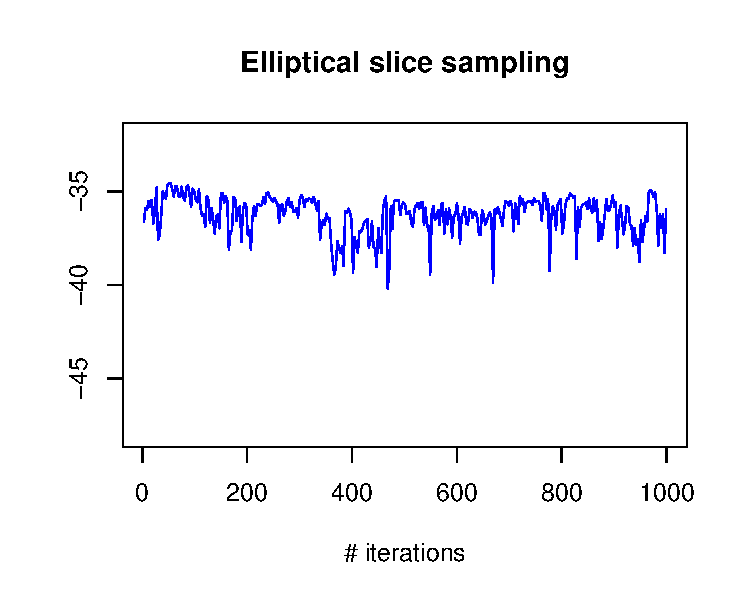
\includegraphics[width = 10cm]{figure1.pdf}
%\caption{Trace plot of log likelihood of 333 points in the first 1000 iterations by taking every 3 iterations}
%\end{figure} 
%\begin{figure}[h!]
%\centering
%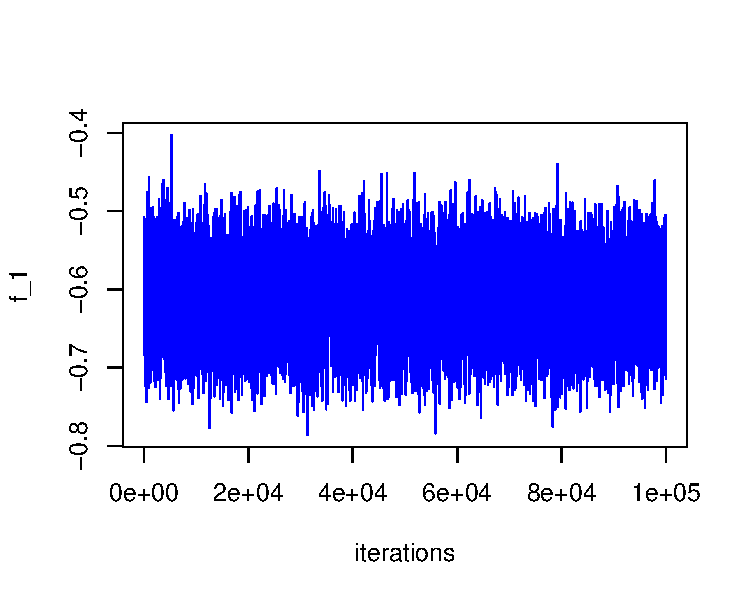
\includegraphics[width = 10cm]{tracef_1.pdf}
%\caption{Trace plot of the first dimension dimension of output $f$ of 100000 iterations}
%\end{figure}
%The traces of log-likelihoods and the first dimension of outputs for $D=1$ are shown in Figure 3 and 4 respectively, which reveal frequent jumps in both chains. The effective sample size for it is 3177.

\subsubsection{Log Gaussian Cox process}

Data of mining disasters are provided by Jarrett et al. \cite{Jarrett}. There were 191 events happening during 40550 days which were partitioned into 811 bins each of which contains 50 days according to Murray, Adams and MacKay $\cite{MAM}$. This means $f$ is 811 dimensional, we notice that both Elliptical Slice Samping and metropolis hastins method take a long time. This makes it harder to validate algorithms on this model. Hence, we partition the period into 102 intervals, such that each interval includes 400 days (except the last one, which is consist of 150 days). Given the date of every event, the number of event happened in each bin can be computed, i.e. $y_n$. Let $l=13516$, $\sigma_f^2 = 1$, $N = 102$, $D=1$ and $m=log(191/102)$. We observe frequent jumps in trace plot and the autocorrelation function goes to 0 within ?? lag(??).
%\begin{figure}[h!]
%\centering
%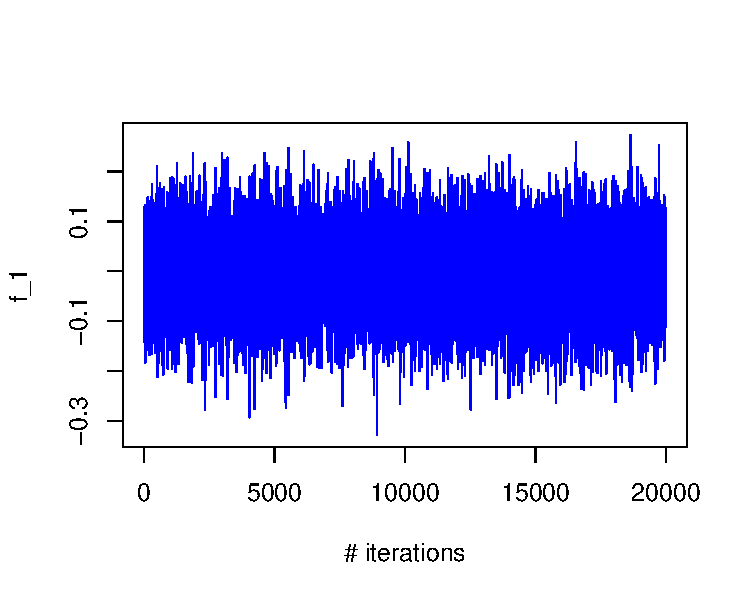
\includegraphics[width = 10cm]{figureminedata.pdf}
%\caption{Trace plot of the first dimension dimension of output $f$ of 20000 iterations}
%\end{figure}

\subsubsection{Comparison}
For Gaussian regression model, we will compare the performance of Elliptical Slice Sampling algorithm with the theorethical Bayesian model, the Metropolis-Hasting algorithm introduced by Neal \cite{Neal} and an adapted Metropolis-Hastings algorithm proposed by Roberts et al. in \cite{Roberts}. 

In order to plot and compare the densities, we restricted the full $4$-models comparison on the $2$-dimensional case. Hence, $N=1$, $D=2$ and, as suggested in \cite{MAM}, we put $\sigma_n=0.3$, $\sigma_f=1$ and $l=1$.
The full Bayesian model will look like this:
\begin{align*}
\mathbf{f}&\sim \mathcal{N}\left(\mathbf{0},\Sigma\right)\\
\mathbf{y}|\mathbf{f}&\sim\mathcal{N}\left(\mathbf{f},\Sigma^{'}\right)\\
\mathbf{f^'}&\sim\mathcal{N}\left(\left(\Sigma^{-1}+\Sigma^{'}^{-1}\right)^{-1}\Sigma^{'}^{-1}\mathbf{y},\left(\Sigma^{-1}+\Sigma^{'-1}\right)^{-1}\right)
\end{align*}
where $\Sigma$, as proposed before, is such that $\Sigma_{i,j}=\text{exp}\left(-\frac{1}{2}\sum_{d=1}^{2}(x_{d,i} - x_{d,j})^2\right)\,i,j=1,2$ and $\Sigma^{'}=\begin{bmatrix}0.09 & 0 \\ 0 & 0.09\end{bmatrix}$.
We tested the normality of these samples with the `mvnorm.skew.test` from the `ICS` pckage and the null hypothesis was not rejected.

For Neal's Metropolis Hastings algorithm, we discover that the performance of the MCMC chain is sensitive to the value of step-size $\epsilon$ because the mixture and convergence of the chain depend on $\epsilon$. We take $\epsilon = 0.2$ after trails of different values. 

With the same target distribution, adaptive Metropolis-Hastings use proposals for $n^{th}$ iteration as follows:\\
\begin{equation}
    q_n(\bf{f},\bf{f'}) = 
    \begin{cases}
     N(\bf{f},(0.1^2)I_d/d) & n\leq 2d \\
        (1-\beta)N(\bf{f},(2.38^2)\Sigma_n/d) + \beta N(\bf{f},(0.1^2)I_d/d) & n > 2d \\
    \end{cases}
\end{equation}

where $\Sigma_n$ is the empirical estimate of the covariance of the target distribution based on the run so far and $\beta$ is a small positive constant \cite{Gareth}.

Compared to other algorithms, Adaptive Metropolis Hastings algorithm takes longer time to reach a stationary variance and good mixture. To avoid complexity of estimating $\Sigma_n$, in this example, we simply take the covariance of the posterior distribution, which is known. In this case, it is not nessary to take the weighted sum as proposal according to previous research \cite{Gareth}. Then the proposal turns out to be $N(\bf{f},(2.38^2)\left(\Sigma^{-1}+\Sigma^{'-1}\right)^{-1}\right/d)$.

In the figure \ref{comparison} we can compare the contour plots of the four samples coming from the theoretical model, the ESS algorithm, the Neal MH and the Adaptive MH. The number of samples for each model was $100000$. It is evident that the stationary distributions of the three algorithms are the correct one.
\begin{figure}[h]\label{comparison}
\centering
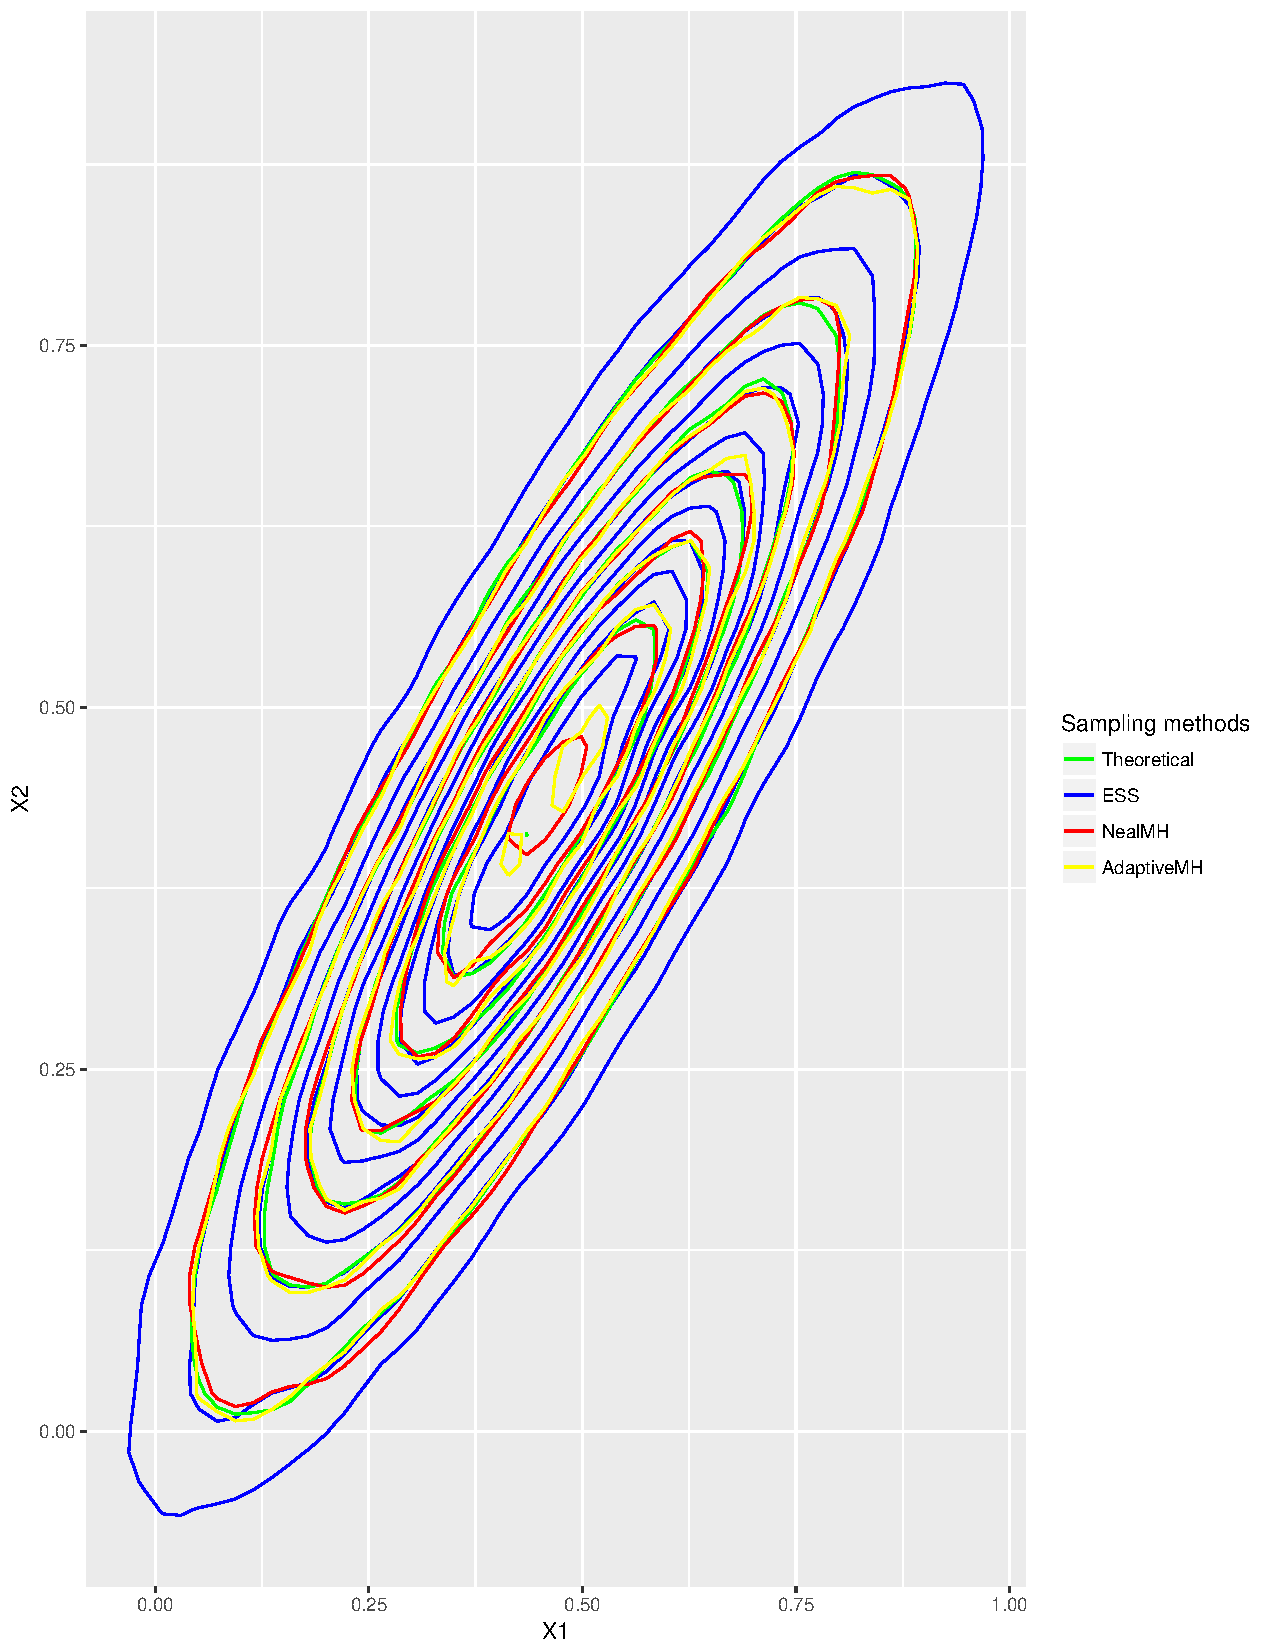
\includegraphics[height=13cm,width = 15cm]{ComparisonGauss.pdf}
\caption{Comparison of contour plots for Gaussian regression}
\end{figure}
%We need to mention the fact that the we tried different step-size parameters for Neal's algorithm to obtain a Gaussian sample. (mentioned)

Then we compare Elliptical Slice Sampling with Neal's MH in terms of effective sample size and CPU time. We run $10^6$ iterations and remove the first $10^5$ burn-in. We encountered problems when implementing Adaptive MH with proposal as shown in Equation (6), which is resulted from the empirical estimation of the covariance matrix. In addition, the update of state is infrequent. In the first 400 iterations, $\bf{f}$ still stay in the same state. Therefore, we only compare Elliptical Slice sampling with Neal's MH. The results are shown in Table 1, which show that Elliptical slice sampling is more efficient compared to Neal's MH because the former one has more effective samples in all 3 examples. The effective samples occupy approximately 47\% for Elliptical slice sampling method while consists of only 21\% of total samples for Neal's MH. The effective sample size is much smaller for data where $\bf{f}$ is 200 dimensional where input vector is 10 dimensional. On the other hand, the elliptical slice sampling takes longer time. But the effective samples per unit time for Elliptical Slice Sampling is larger in general. For example, for $R1$, the effective samples per unit time is 2.1 for Elliptical Slice Sampling, which is approximately twice as large as Neal's MH.

\begin{table}[!htbp]
\centering
\caption{Compare Elliptical Slice Sampling with Neal's Metropolis Hastings on data $R1$, $R10$ and $Mining$ in terms of effective sample size and CPU time.}
\begin{tabular}{*7c}
\toprule
 {} &  \multicolumn{2}{c}{R1} & \multicolumn{2}{c}{R10} & \multicolumn{2}{c}{Mining}\\
\midrule
{}   & ESS   & NMH    & ESS   & NMH  & ESS   & NMH\\
effective samples   &  33316.79 & 13330.98   & 2139.793  & 1159.535 & 429181.7 & 186571\\
CPU time   &  15898.001 & 9472.684   & 16374.79  & 10497.30 & 3448.755 & 3271.421\\

\bottomrule

\end{tabular}
\end{table}

\section{Discussion and Conclusion}

Neal's MH requires extra time to tune step-size. Combined the results discovered in Section 3, Elliptical Slice Sampling outperforms Neal's MH in terms of time complexity, efficiency and mixture of Markov chains (??).
\begin{thebibliography}{12}


\bibitem{Jarrett}
	Jarrett, R. G.  (1979)
	\emph{A note on the intervals between coal-mining disasters},
	Biometrika.

\bibitem{Moller}
	M{\o}ller, J., Syversveen, A. R., Waagepetersen  (1998)
	\emph{Log Gaussian Cox processes},
	Scandinavian Journal of Statistics.

\bibitem{MAM}
	Murray, I., Adams, R. P., and MacKay, D. J. C. (2010)
	\emph{Elliptical slice sampling},
	Journal of Machine Learning Research.
	
\bibitem{Neal}
	Neal, R. M. (1999)
	\emph{Regression and Classification Using
Gaussian Process Priors},
	Bayesian Statistics 6 (475-501), OU Press.
	
\bibitem{Neal2003}
	Neal, R. M. (2003)
	\emph{Slice sampling},
	Annals of Statistics.

\bibitem{Roberts}
	Roberts, G. O., Rosenthal, J. S. (2009)
	\emph{Examples of Adaptive MCMC},
	Journal of Computational and Graphical Statistics.
	
\bibitem{Gareth} Gareth O. Roberts & Jeffrey S. Rosenthal (2009) \emph{Examples of Adaptive MCMC}, Journal of COmputational and Graphical Statistics, 18:2, 349-367, DOI:10.1198/icgs.2009.06134.

\end{thebibliography}

\end{document}








